\section{Plugin System and the MathNetwork Plugin}
\label{sec:plugins}

The core data model (\S\ref{sec:data-model}) is domain-agnostic: it stores entries with refs and records but does not interpret their meaning. To do useful work, we need plugins that impose domain-specific conventions. In this section, we present the \textbf{MathNetwork} plugin, which turns Astrolabe into a bridge between informal and formal mathematics.

\paragraph{The gap between blueprint and formalization.}

In Lean~4, the \texttt{leanblueprint} tool provides a visual dependency graph for formalization projects. Dependencies are declared via \LaTeX\ macros (\verb|\uses{lem:foo}|), but each edge carries only the label ``uses.'' On the other side, the Lean compiler produces a fine-grained declaration-level dependency graph --- but again, edges carry no semantic content.

\begin{figure}[ht]
\centering
\begin{tikzpicture}[
  bp/.style={draw, rounded corners=2pt, fill=green!10, font=\scriptsize, inner sep=3pt, minimum width=1.4cm, minimum height=0.5cm},
  decl/.style={circle, fill, inner sep=1.5pt},
  arr/.style={->, >=Stealth, thin},
  darr/.style={->, >=Stealth, thin, red!60!black}
]
% Left: Blueprint graph
\node[font=\small\bfseries] at (1.5, 2.8) {Blueprint};
\node[bp] (la) at (1.5, 2) {\texttt{length\_append}};
\node[bp] (lm) at (0, 0.5) {\texttt{length\_map}};
\node[bp] (mm) at (3, 0.5) {\texttt{map\_map}};
\node[bp] (len) at (1.5, -0.8) {\texttt{List.length}};
\draw[arr] (la) -- node[left, font=\tiny] {uses} (lm);
\draw[arr] (la) -- node[right, font=\tiny] {uses} (len);
\draw[arr] (lm) -- node[left, font=\tiny] {uses} (len);
\draw[arr] (mm) -- node[right, font=\tiny] {uses} (len);

% Right: Declaration-level graph
\node[font=\small\bfseries] at (7.5, 2.8) {Declaration graph};
\node[decl, label={[font=\scriptsize]above:\texttt{length\_append}}] (a) at (7.5, 2) {};
\node[decl, label={[font=\scriptsize]left:\texttt{length\_map}}] (b) at (5.8, 0.8) {};
\node[decl, label={[font=\scriptsize]right:\texttt{map\_map}}] (c) at (9.2, 0.8) {};
\node[decl, label={[font=\scriptsize]below:\texttt{List.length}}] (d) at (7.5, -0.3) {};
\node[decl, label={[font=\scriptsize]left:\texttt{List.rec}}] (rec) at (5.5, -0.5) {};
\node[decl, label={[font=\scriptsize]right:\texttt{Nat.add}}] (add) at (9.5, -0.5) {};
\node[decl, label={[font=\scriptsize]below:\texttt{List.map}}] (map) at (7.5, -1.3) {};
\draw[darr] (a) -- (b);
\draw[darr] (a) -- (d);
\draw[darr] (a) -- (add);
\draw[darr] (b) -- (d);
\draw[darr] (b) -- (map);
\draw[darr] (c) -- (map);
\draw[darr] (c) -- (rec);
\draw[darr] (d) -- (rec);
\draw[darr, dashed, gray] (a) to[bend right=15] (rec);
\draw[darr, dashed, gray] (a) to[bend left=15] (map);
\end{tikzpicture}
\caption{Left: a \texttt{leanblueprint} dependency graph. Each edge is labeled ``uses'' with no further content. Right: a declaration-level dependency graph extracted from Lean~4 compilation artifacts. Both representations lose the \emph{semantic content} of each edge.}
\label{fig:blueprint-vs-decl}
\end{figure}

Neither representation captures \emph{how} a dependency is used. Astrolabe's data model solves this: every edge is itself an entry with a full \texttt{record}, so the nature of each dependency can be explicitly described.

\paragraph{Network extraction.}
The MathNetwork plugin requires a convention on the entry store: the network is built from entries of degree~0 and degree~1 only. Atoms (degree~0) become \emph{nodes}. Degree-1 entries whose two refs are both atoms become \emph{directed edges} ($\texttt{ref[0]} \to \texttt{ref[1]}$), with edge semantics derived from the record's \texttt{sort} field. Figure~\ref{fig:entry-view} shows the entry view; Figure~\ref{fig:network-view} shows the extracted network.

\begin{figure}[ht]
\centering
\begin{minipage}[t]{0.48\textwidth}
\vspace{0pt}
\centering
\scalebox{1.3}{%
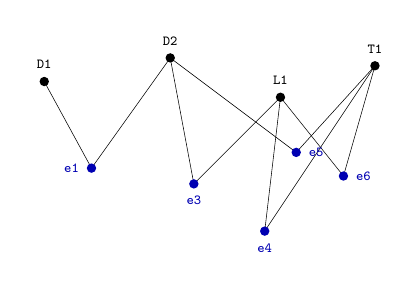
\begin{tikzpicture}[v/.style={circle, fill, inner sep=0.5pt}]
  \tikzset{s0/.style={circle, fill=black, inner sep=1.2pt}}
  \tikzset{s1/.style={circle, fill=blue!70!black, inner sep=1.2pt}}
  % links
  \draw[very thin] (0.6,1.3) -- (0.0,2.4);
  \draw[very thin] (0.6,1.3) -- (1.6,2.7);
  \draw[very thin] (1.9,1.1) -- (1.6,2.7);
  \draw[very thin] (1.9,1.1) -- (3.0,2.2);
  \draw[very thin] (3.2,1.5) -- (1.6,2.7);
  \draw[very thin] (3.2,1.5) -- (4.2,2.6);
  \draw[very thin] (2.8,0.5) -- (3.0,2.2);
  \draw[very thin] (2.8,0.5) -- (4.2,2.6);
  \draw[very thin] (3.8,1.2) -- (4.2,2.6);
  \draw[very thin] (3.8,1.2) -- (3.0,2.2);
  % atoms
  \node[s0] (D1) at (0.0,2.4) {};
  \node[font=\tiny, above=1pt] at (D1) {\texttt{D1}};
  \node[s0] (D2) at (1.6,2.7) {};
  \node[font=\tiny, above=1pt] at (D2) {\texttt{D2}};
  \node[s0] (L1) at (3.0,2.2) {};
  \node[font=\tiny, above=1pt] at (L1) {\texttt{L1}};
  \node[s0] (T1) at (4.2,2.6) {};
  \node[font=\tiny, above=1pt] at (T1) {\texttt{T1}};
  % degree-1 entries
  \node[s1] (e1) at (0.6,1.3) {};
  \node[font=\tiny, left=1pt, text=blue!70!black] at (e1) {\texttt{e1}};
  \node[s1] (e3) at (1.9,1.1) {};
  \node[font=\tiny, below=1pt, text=blue!70!black] at (e3) {\texttt{e3}};
  \node[s1] (e4) at (2.8,0.5) {};
  \node[font=\tiny, below=1pt, text=blue!70!black] at (e4) {\texttt{e4}};
  \node[s1] (e5) at (3.2,1.5) {};
  \node[font=\tiny, right=1pt, text=blue!70!black] at (e5) {\texttt{e5}};
  \node[s1] (e6) at (3.8,1.2) {};
  \node[font=\tiny, right=1pt, text=blue!70!black] at (e6) {\texttt{e6}};
\end{tikzpicture}%
}
\end{minipage}%
\hspace{4pt}%
\begin{minipage}[t]{0.48\textwidth}
\vspace{0pt}
{\scriptsize\ttfamily
\begin{tabular}{@{}l@{}}
\{\\
\ \ \textcolor{black}{"D1"}:\{"ref":["\textcolor{black}{D1}"],"record":"definition ..."\},\\
\ \ \textcolor{black}{"D2"}:\{"ref":["\textcolor{black}{D2}"],"record":"definition ..."\},\\
\ \ \textcolor{black}{"L1"}:\{"ref":["\textcolor{black}{L1}"],"record":"lemma ..."\},\\
\ \ \textcolor{black}{"T1"}:\{"ref":["\textcolor{black}{T1}"],"record":"theorem ..."\},\\
\ \ \textcolor{blue!70!black}{"e1"}:\{"ref":["\textcolor{black}{D2}","\textcolor{black}{D1}"],\\
\ \ \ \ \ \ "record":"D2 uses D1"\},\\
\ \ \textcolor{blue!70!black}{"e3"}:\{"ref":["\textcolor{black}{D2}","\textcolor{black}{L1}"],\\
\ \ \ \ \ \ "record":"L1 depends on D2"\},\\
\ \ \textcolor{blue!70!black}{"e4"}:\{"ref":["\textcolor{black}{L1}","\textcolor{black}{T1}"],\\
\ \ \ \ \ \ "record":"T1 cites L1"\},\\
\ \ \textcolor{blue!70!black}{"e5"}:\{"ref":["\textcolor{black}{D2}","\textcolor{black}{T1}"],\\
\ \ \ \ \ \ "record":"T1 unfolds D2"\},\\
\ \ \textcolor{blue!70!black}{"e6"}:\{"ref":["\textcolor{black}{T1}","\textcolor{black}{L1}"],\\
\ \ \ \ \ \ "record":"T1 applies L1"\}\\
\}
\end{tabular}
}
\end{minipage}
\caption{Entry view: \textcolor{black}{black} = atoms (D1, D2, L1, T1), \textcolor{blue!70!black}{blue} = degree-1 entries (e1--e5) carrying open-ended semantic records.}
\label{fig:entry-view}
\end{figure}

\begin{figure}[ht]
\centering
\scalebox{2.0}{%
\begin{tikzpicture}[v/.style={circle, fill, inner sep=0.5pt}]
  \tikzset{s0/.style={circle, fill=black, inner sep=1.2pt}}
  % atoms
  \node[s0] (D1) at (0.0,1.4) {};
  \node[font=\tiny, left=1pt] at (D1) {\texttt{D1}};
  \node[s0] (D2) at (1.8,2.2) {};
  \node[font=\tiny, above=1pt] at (D2) {\texttt{D2}};
  \node[s0] (L1) at (3.4,0.8) {};
  \node[font=\tiny, below=1pt] at (L1) {\texttt{L1}};
  \node[s0] (T1) at (4.8,2.0) {};
  \node[font=\tiny, right=1pt] at (T1) {\texttt{T1}};
  % e1: D2 -> D1
  \draw[->, >=Stealth, very thin, blue!70!black] (D2) -- (D1);
  \node[font=\tiny, text=blue!70!black] at (0.7,2.0) {e1};
  % e3: D2 -> L1
  \draw[->, >=Stealth, very thin, blue!70!black] (D2) -- (L1);
  \node[font=\tiny, text=blue!70!black, left=1pt] at (2.5,1.4) {e3};
  % e5: D2 -> T1
  \draw[->, >=Stealth, very thin, blue!70!black] (D2) -- (T1);
  \node[font=\tiny, text=blue!70!black, above=1pt] at (3.3,2.2) {e5};
  % e4: L1 -> T1 (slight bend up)
  \draw[->, >=Stealth, very thin, blue!70!black, bend left=15] (L1) to (T1);
  \node[font=\tiny, text=blue!70!black] at (3.9,1.7) {e4};
  % e6: T1 -> L1 (slight bend down)
  \draw[->, >=Stealth, very thin, blue!70!black, bend left=15] (T1) to (L1);
  \node[font=\tiny, text=blue!70!black] at (4.5,1.1) {e6};
\end{tikzpicture}%
}
\caption{Network view of the same knowledge base. Atoms become nodes; degree-1 entries become directed edges ($\texttt{ref[0]} \to \texttt{ref[1]}$). Edge labels (e1--e5) correspond to the entries in Figure~\ref{fig:entry-view}.}
\label{fig:network-view}
\end{figure}

The following two subsections define the record conventions for informal and formal mathematics that this plugin expects.

\paragraph{Informal mathematics: \texttt{source: "tex"}.}

For informal mathematical content, the \texttt{sort} field is derived from the \LaTeX\ environment (e.g., \verb|\begin{theorem}| $\to$ \texttt{sort: "theorem"}). The record carries the mathematical statement in natural language:

\medskip
{\scriptsize\ttfamily
\begin{tabular}{@{}l@{}}
\{"sort":"definition", "source":"tex", "title":"Compact Space",\\
\ \ "notes":"A subset $K$ is compact if every open cover has a finite subcover."\}\\[4pt]
\{"sort":"theorem", "source":"tex", "title":"Heine-Borel",\\
\ \ "notes":"A subset of $\mathbb{R}^n$ is compact iff it is closed and bounded."\}
\end{tabular}
}
\medskip

Atoms are definitions, theorems, lemmas, propositions, corollaries, and examples. Higher-degree entries represent relationships between them: a proof references the theorem it proves and the lemmas it uses. The \texttt{notes} field supports \LaTeX\ math and inline references via \verb|\entryref{hash}{text}|.

\paragraph{Formal mathematics: \texttt{source: "lean"}.}

For formal mathematics, the \texttt{sort} field mirrors the Lean keyword (\texttt{def} $\to$ \texttt{definition}, \texttt{theorem} $\to$ \texttt{theorem}). The \texttt{content} field stores the source code, and \texttt{state} tracks formalization progress:

\medskip
{\scriptsize\ttfamily
\begin{tabular}{@{}l@{}}
\{"sort":"theorem", "source":"lean", "title":"List.length\_append",\\
\ \ "state":"proven", "content":"theorem length\_append (l1 l2 : List a) : ..."\}\\[4pt]
\{"sort":"definition", "source":"lean", "title":"List.length",\\
\ \ "state":"proven", "content":"def length : List a -> Nat | [] => 0 | ..."\}
\end{tabular}
}
\medskip

Formal dependencies can be generated automatically by a source plugin that parses Lean's compilation artifacts. Unlike \texttt{leanblueprint} or declaration graphs, Astrolabe edges carry open-ended content --- a dependency can record not just ``uses'' but ``rewrites by,'' ``unfolds definition of,'' or ``applies to subterm.''

\paragraph{Edges and cross-source correspondence.}

Edges (degree-1 entries) connect two atoms. Their sort is auto-derived from the pair of source sorts:

\begin{table}[H]
\centering
\begin{tabular}{ll}
\toprule
Edge sort pair & Meaning \\
\midrule
\texttt{(theorem, proof)} & Statement--proof link \\
\texttt{(theorem, definition)} & Depends on definition \\
\texttt{(proof, lemma)} & Proof cites lemma \\
\texttt{(theorem, theorem)} & Cross-source correspondence \\
\bottomrule
\end{tabular}
\end{table}

When both \texttt{tex} and \texttt{lean} entries coexist in the same file, a \texttt{(theorem, theorem)} edge with one \texttt{tex} source and one \texttt{lean} source marks the formalization correspondence. This makes the bridge between informal and formal mathematics explicit and navigable in the network view.

\paragraph{Semantic propagation.}
The entry-level hash propagation (\S\ref{sec:data-model}) maintains data integrity: when an atom changes, all degree-1 entries referencing it are re-hashed. But this does not capture \emph{semantic} dependency. Consider: Definition~$D$ changes; Edge~$E$ (``Theorem~$T$ depends on~$D$'') is re-hashed because its ref contains~$D$; but Theorem~$T$ itself is unaffected --- its ref is $[\text{self}]$ and its record may not mention~$D$'s hash. To address this, the MathNetwork plugin adds a second layer of propagation on the skeleton graph: when an atom changes, the directed edge structure is traversed in reverse to identify all atoms that \emph{semantically} depend on the changed atom. If Definition~$D$ is modified, every atom reachable by following edges backward from~$D$ is flagged as affected. This is a straightforward reverse BFS on the skeleton graph.
